\chapter{Introduction [AS PER SCOPE DOCUMENT]}
\label{sec:introduction}
The "Introduction" section sets the foundation for the entire report and should be carefully crafted to give the reader a clear understanding of the project’s scope, objectives, and context. Here’s what you can include:

Background:

Begin by providing background information on the broader topic or field your development project is related to.
Highlight any existing problems, gaps, or opportunities that led to the motivation for your project.
Include relevant references to previous research, development projects, or technologies. For example, you might want to cite studies or prior systems that failed to address the issues you're focusing on.


\section{Existing Solutions}

For the Existing Solutions section, students should research and describe various solutions, methods, or approaches that have been previously developed to solve the problem they are addressing. This section should include an overview of the different techniques, technologies, or models that are currently in use or have been applied in the past. Students should critically assess the strengths and weaknesses of each solution, highlighting any gaps or limitations that their project aims to address. Additionally, this section should show an understanding of the state-of-the-art in the field and provide context for why the proposed solution is necessary or an improvement over existing ones.


\begin{table}[H]
\centering
\caption{Comparison of Existing Solutions}
\begin{tabular}{|c|p{5cm}|p{5cm}|}
\hline
\textbf{System Name}   & \textbf{System Overview} & \textbf{System Limitations} \\ \hline
System 1               & Brief description of what System 1 does and its primary features. & Highlight the shortcomings or issues with System 1. \\ \hline
System 2               & Brief description of what System 2 does and its primary features. & Highlight the shortcomings or issues with System 2. \\ \hline
System 3               & Brief description of what System 3 does and its primary features. & Highlight the shortcomings or issues with System 3. \\ \hline
\end{tabular}
\label{tab:system_comparison}
\end{table}

\section{Problem Statement}
Academic dishonesty has become a significant concern in educational institutions worldwide. 
Studies indicate that approximately 61\% of university students have admitted to cheating during written examinations, 
while nearly 68\% confess to cheating at least once during their academic career \cite{bucciol2020cheating}. 
Traditional manual invigilation methods are often insufficient, as invigilators may unintentionally overlook suspicious activities, 
and reviewing long hours of CCTV/camera footage after exams is both time-consuming and ineffective.

To address these challenges, \textbf{ForeSyte} provides an AI-driven solution for automated examination monitoring. 
The system processes both real-time CCTV/camera streams and uploaded video footage, detecting suspicious activities such as 
phone usage, hand waving, bending over the desk, looking around, and standing up using advanced computer vision techniques.

The system focuses on seat-specific mapping, ensuring that every detected activity is linked to the correct student. 
It also ensures that the correct student ID is sitting on the assigned seat by using face recognition.  
In addition, \textbf{ForeSyte} incorporates an Invigilator Activity Monitoring module to:
\begin{itemize}
    \item Track invigilators' movements
    \item Detect prolonged idle periods
    \item Identify potential negligence
\end{itemize}
An admin dashboard provides real-time monitoring and automated report generation, enabling discipline committees to 
directly access timestamped violations instead of manually searching through hours of footage. 
By combining AI-powered surveillance with intelligent analytics, \textbf{ForeSyte} enhances exam security and aims to 
reduce academic dishonesty over time by providing actionable insights. Furthermore, as students become aware that their activities 
are continuously monitored and every suspicious action is captured with timestamped reports, the likelihood of cheating 
is expected to decrease significantly over repeated examination sessions

\begin{figure}[H]
    \centering
     \caption{Estimated reduction in cheating rates using ForeSyte AI-based surveillance system}
    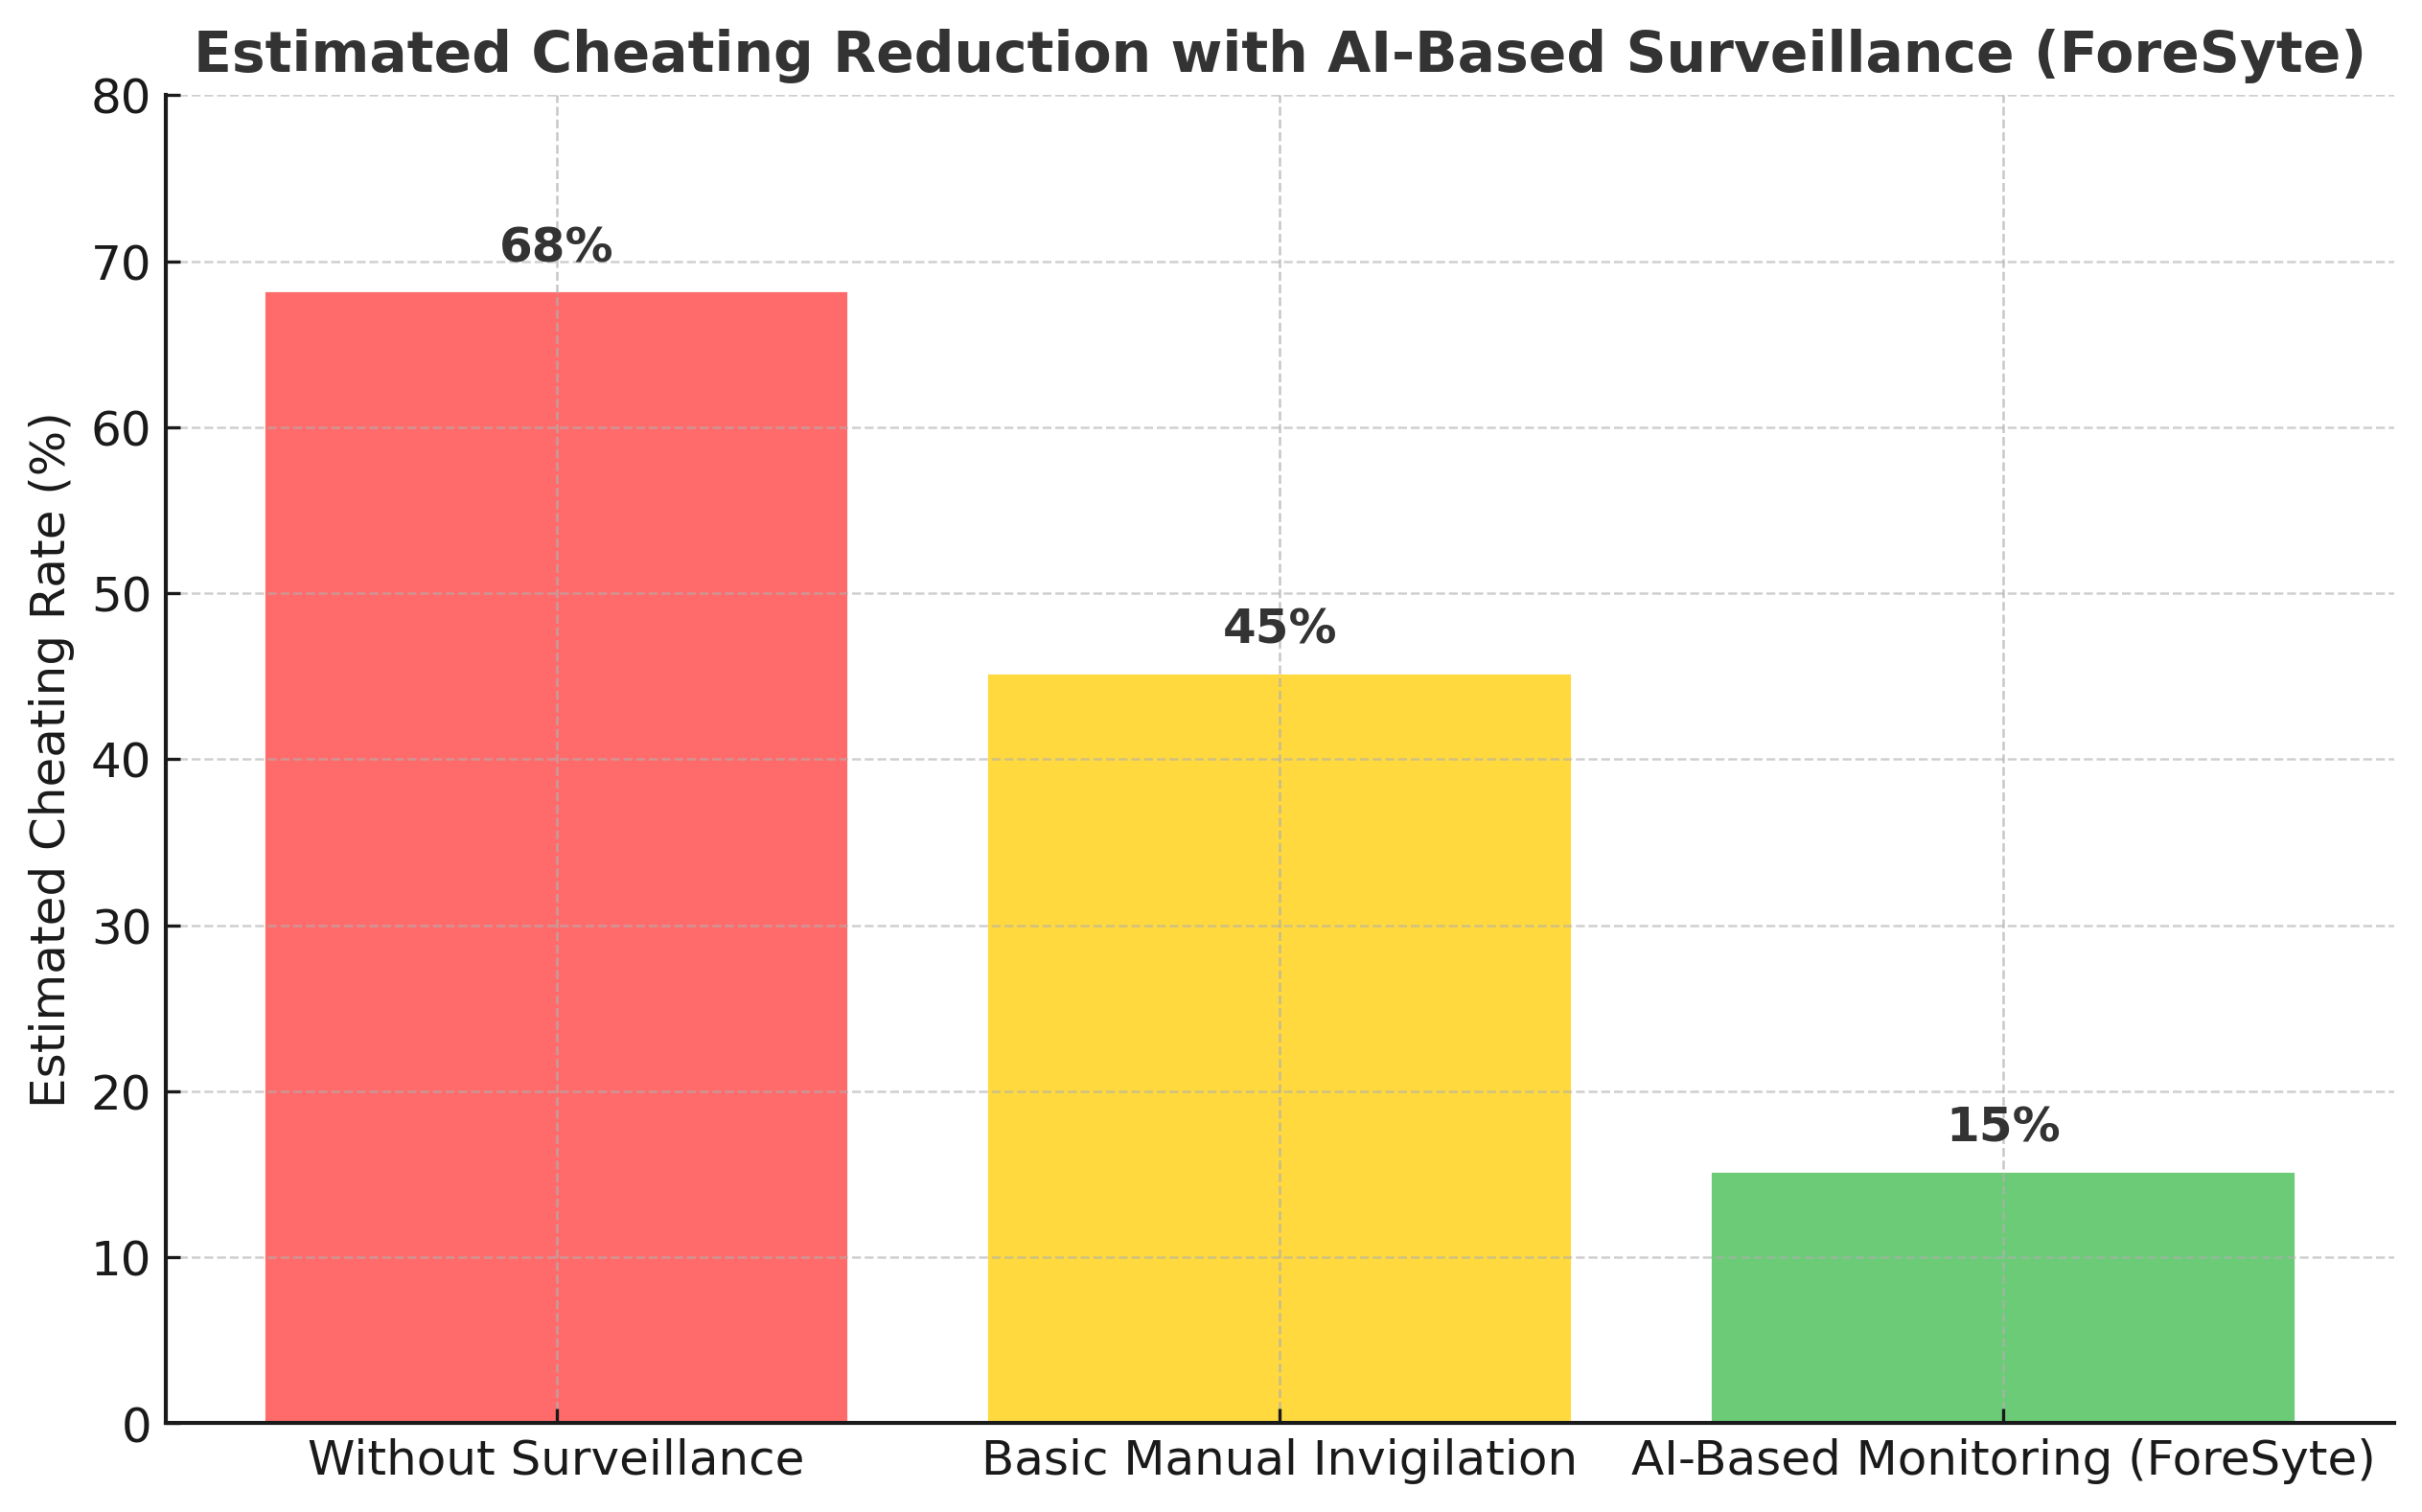
\includegraphics[width=0.8\linewidth]{sections/cheating_reduction_foreSyte.png}
    \label{fig:cheating_reduction}
\end{figure}

\begin{figure}[H]
    \centering
    \caption{Frequency of students who reported cheating during written examinations \cite{bucciol2020cheating}}
    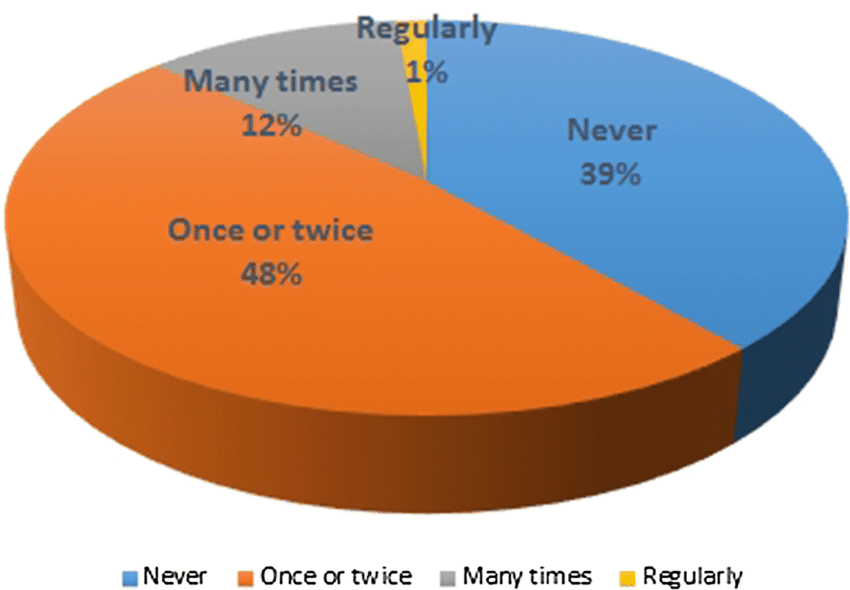
\includegraphics[width=0.7\linewidth]{sections/piechart.png}
    \label{fig:cheating_frequency}
\end{figure}
\FloatBarrier
\section{Scope}
The scope of the ForeSyte project includes developing an AI-powered exam surveillance 
system that enhances the integrity of examinations conducted in physical exam halls. 
Recent research highlights the importance of automated invigilation for maintaining 
academic integrity \cite{bucciol2020cheating, examIntegrity2021}. 

\begin{figure}[h]
    \centering
    \caption{Scope workflow of the ForeSyte system}
    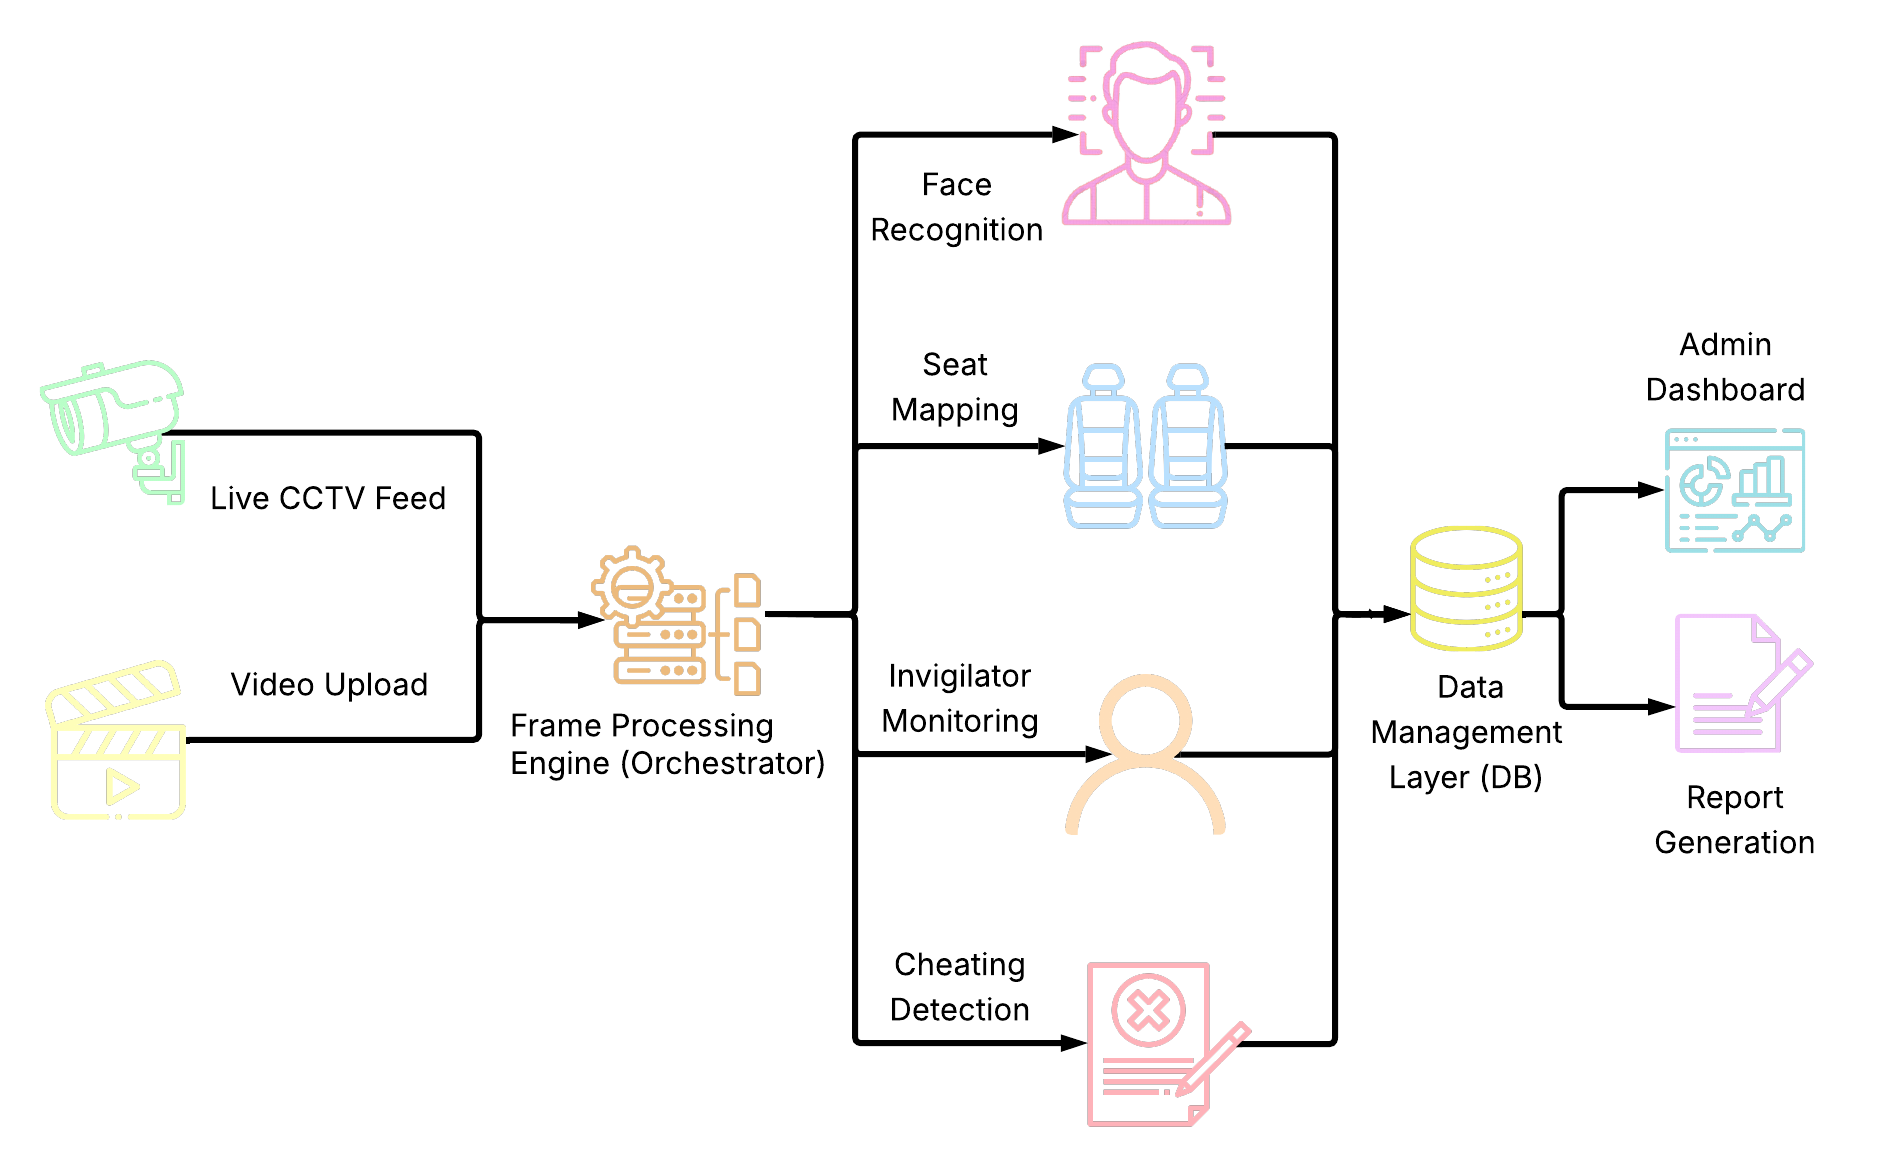
\includegraphics[width=0.9\textwidth]{sections/flowchart.png}
    \label{fig:flowchart}
\end{figure}

The system will process CCTV/camera footage, both live streams and uploaded recordings, to 
automatically detect and log suspicious activities such as unauthorized object usage and 
irregular gestures. It will also incorporate seating arrangement verification, ensuring that 
each detected activity is accurately linked to the correct student, and that the correct student ID 
is sitting in the assigned seat using face recognition, similar to approaches in modern proctoring systems \cite{masud2025cheating_detection, arumugam2025smart_invigilation}. 

The project further extends to monitoring invigilator activity within the exam hall, 
identifying negligence or prolonged absence from duty. Similar works on offline and 
intelligent monitoring systems support this approach \cite{holi2025iems, moyo2023openpose_exam_detection}. 
All detected events will be recorded with precise timestamps, seat numbers and room 
identifiers, enabling a structured and transparent record of violations.

An administrative dashboard will be developed to centralize monitoring and provide 
clear violation reports supported with visual evidence. This will reduce the need for 
institutions to manually review extensive CCTV/camera footage, offering instead a concise and 
accurate summary of flagged incidents. 

The system will be designed for real-time performance using optimized frame sampling 
and AI models capable of efficient video analysis. The project will be self-funded and 
developed entirely by our team. Related research also discusses the ethical implications of 
AI in exam supervision, highlighting fairness and privacy issues. 

The boundaries of this project are confined to creating a robust and intelligent surveillance 
solution that automates detection, verification, and reporting within physical exam 
environments, thereby ensuring greater fairness, efficiency, and accountability in academic assessments.
\section{Modules} 

The \textbf{ForeSyte} project is organized into several core modules, each responsible for specific functionalities required to ensure seamless, automated exam monitoring. 
The modules are divided into two main components: the \textit{ForeSyte Web Portal} for stakeholders and the \textit{Backend Service} that powers the AI-driven monitoring capabilities.

\subsection{ForeSyte Web Portal}
The \textbf{ForeSyte Web Portal} is a multi-user interface designed for administrators, discipline committee members, and university management. 
It provides centralized access to seating plans and violation reports, ensuring transparent and efficient management of examination activities.

\begin{enumerate}
    \setlength{\itemsep}{2pt}
    \item \textbf{Dashboard Visualization:} Displays real-time updates of suspicious activities, flagged violations, and invigilator presence across multiple exam halls using data from connected CCTV/camera systems.
    \item \textbf{Report Access:} Enables authorized users to view, manage, and download detailed violation reports containing timestamps, seat details and room information.
    \item \textbf{User Roles and Permissions:} Implements secure role-based access, where administrators manage seating plans, camera configurations, and exam schedules, while discipline committee members focus on reviewing reports and initiating actions.
    \item \textbf{Seating Plan Integration:} Links violations to student seating layouts and verifies correct student IDs using face recognition to ensure accurate identification of candidates involved in flagged incidents.
\end{enumerate}

\subsection{Backend Service}
The \textbf{Backend Service} powers the core intelligence of the ForeSyte system, managing video analysis, behavioral detection, invigilator monitoring, and reporting. 
This module processes video streams from CCTV/camera systems and uploaded exam footage to ensure accurate real-time and recorded exam monitoring.

\begin{enumerate}
    \setlength{\itemsep}{2pt}
    \item \textbf{Video Stream Processing:} Integrates with CCTV/camera systems and uploaded recordings, extracting frames for real-time detection of activities and events.
    \item \textbf{Cheating Detection Engine:} Uses advanced computer vision techniques to identify suspicious behaviors such as unauthorized object usage, irregular gestures, communication, and frequent seat movements \cite{bhatti2023smart, arumugam2025smart_invigilation}.
    \item \textbf{Face and Seat Verification:} Verifies student identities and ensures correct student ID is sitting on the assigned seat using face recognition, mapping detected activities to seating plans for accurate violation reporting.
    \item \textbf{Invigilator Monitoring:} Tracks invigilator's prolonged absences from assigned zones, and identifies potential negligence or unauthorized phone usage\cite{moyo2023openpose_exam_detection}.
    \item \textbf{Report Generation:} Compiles timestamped violation logs, including room details, seat numbers, and integrates them directly into the ForeSyte Web Portal for automated PDF/Excel report exports.
\end{enumerate}

\section{Work Division}
For each module and respective feature, responsibility is assigned to a team member.

\begin{table}[!h]
\centering
\begin{tabular}{|l|p{10cm}|}
\hline
\textbf{Name} & \textbf{Responsibility} \\ \hline

Inam Ullah Shaikh & 
\begin{itemize}
    \item Frontend Development
    \item Model Training
    \item Documentation
    \item Deployment
    \item Backend Integration
\end{itemize} \\ \hline

Emaan Fatima & 
\begin{itemize}
    \item Backend Development
    \item Model Research
    \item Model Training
    \item Documentation
    \item Deployment
\end{itemize} \\ \hline

Aden Sial & 
\begin{itemize}
    \item Data Collection
    \item Model Training
    \item Model Research
    \item Documentation
    \item Deployment
\end{itemize} \\ \hline

\end{tabular}
\caption{Work Division among Team Members}
\end{table}

\newpage

